\documentclass[11pt,a4paper]{article}
\usepackage[utf8]{inputenc}
\usepackage{geometry}
\geometry{a4paper, margin=1in}
\usepackage{graphicx}
% Find project images when compiling from reports/module1/, reports/, or root.
\graphicspath{{../../output/}{../output/}{output/}}
\usepackage{float}
\usepackage{hyperref}
\usepackage{booktabs}
\usepackage{amsmath}
\usepackage{xcolor}
% Allow extra line-breaking flexibility for long inline formulas.
\setlength{\emergencystretch}{2em}

\title{Module 1 Report: Core Renderers}
\author{Student Number: S2510156} % 替换为你的考号
\date{\today}

\begin{document}

\maketitle

\section{Introduction and AI Usage Declaration}
% 根据 PDF §1.3 要求，必须声明 AI 使用情况
% TODO (student-authored): distinguish your problem discovery, understanding,
% judgement and actual edits from code generation/changes executed by AI.
% Check the existing tool name and manual-authorship claims against real history.
This report documents the implementation of the Whitted-Style Ray Tracer (WSRT) and Distributed Ray Tracer (DRT) for Module 1.

\textbf{AI Usage Declaration:} I used an AI coding assistant (Claude Sonnet 4.6) to help generate initial boilerplate code for the PBRT parser and the basic ray-sphere intersection logic. I also used it to debug the refraction logic. The core integrator loops, the BRDF implementation, and the BVH (for future modules) were written and modified manually. All rendered images and scene files were created by me. The text of this report was written entirely by me without AI assistance.

\section{WSRT (Whitted-Style Ray Tracer)}

\subsection{Specular Reflection}
\textbf{Design Decisions:} I implemented recursive reflection using the formula \( \mathbf{d}_r = \mathbf{d} - 2(\mathbf{d} \cdot \mathbf{n})\mathbf{n} \). The recursion depth is limited to a configurable maximum (MD=8 for simple, MD=12 for creative) to prevent infinite loops. The throughput is multiplied by the material's reflectance at each bounce.
% 请自行补充：为什么限制递归？反射率如何影响图像？
\textbf{Difficulties Encountered:} Initially, I passed the incident ray direction directly to the reflection function, which caused incorrect shading. I fixed this by ensuring the dot product uses the outward-facing normal. I also fixed a bug where depth termination returned the throughput as radiance, causing false brightness.
\textbf{Example Render:}
\begin{figure}[H]
    \centering
    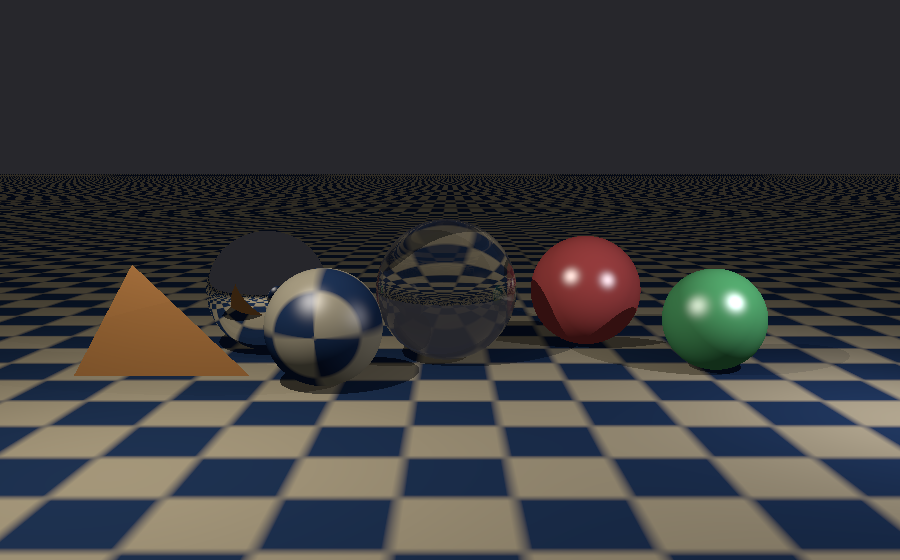
\includegraphics[width=0.8\textwidth]{WSRT_simple.png}
    % Source: output/WSRT_simple.png; scene: scenes/WSRT_simple.pbrt.
    % TODO: this is an unannotated render; add actual arrows/insets.
    \caption{WSRT\_simple. The arrow points to the mirror sphere showing reflections of the floor and other objects.}
    \label{fig:wsrt_simple}
\end{figure}
\textbf{Observations:} The mirror sphere correctly reflects the checkerboard floor.

\subsection{Specular Refraction (Fresnel and TIR)}
\textbf{Design Decisions:} I used Snell's Law (\( \eta_i \sin\theta_i = \eta_t \sin\theta_t \)) and the Fresnel equations to compute the reflection/refraction ratio. Total Internal Reflection (TIR) is handled when \( \sin^2\theta_t \ge 1 \). The medium is determined by checking \( \text{dot}(\mathbf{ng}, \mathbf{ray.d}) < 0 \). The transmission weight is scaled by \( (\eta_i/\eta_t)^2 \).
\textbf{Difficulties Encountered:} I had bugs with the sign of the refraction direction and the handling of the normal when exiting the medium. I also had to fix the DRT integrator which was discarding the weaker Fresnel branch.
\textbf{Example Render:}
\begin{figure}[H]
    \centering
    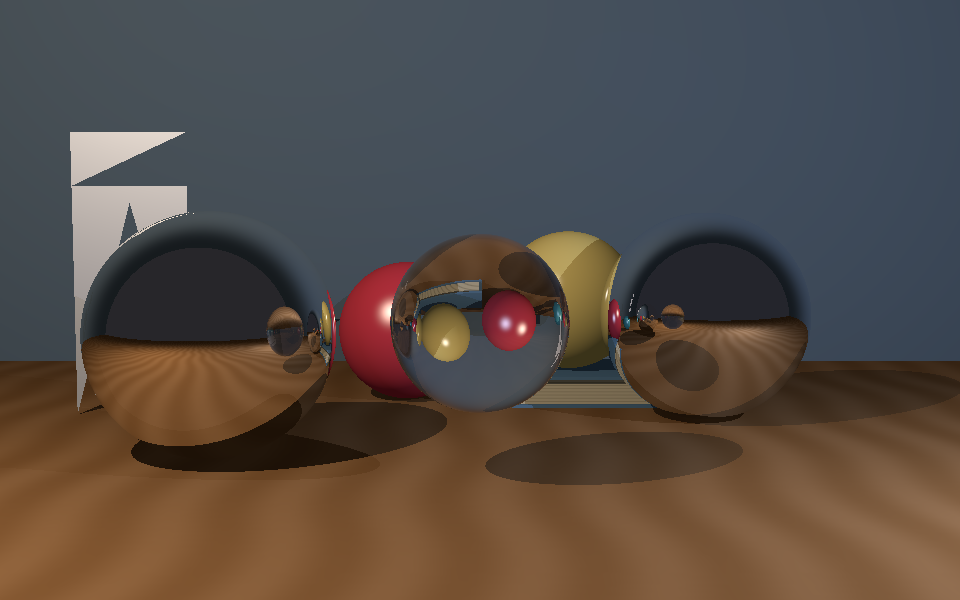
\includegraphics[width=0.8\textwidth]{WSRT_creative.png}
    % Source: output/WSRT_creative.png; actual glass geometry is a scaled sphere.
    % TODO: add your real inspiration photograph and verify reflection claims.
    \caption{WSRT\_creative. The arrow indicates the glass slab where refraction and internal reflection are visible.}
    \label{fig:wsrt_creative}
\end{figure}
\textbf{Observations:} The glass slab (eta=1.60) shows distorted background patterns due to refraction.
% 请自行补充：R/T 随角度如何变化？哪个区域证明折射？

\subsection{Blinn-Phong Shading}
\textbf{Design Decisions:} Ambient is \( \text{baseColor} \times \text{ambientScale} \). Diffuse uses \( \text{baseColor}/\pi \times \max(0, \mathbf{n}\cdot\mathbf{wi}) \times I/r^2 \). Specular uses the half-vector \( \mathbf{h} = \text{normalize}(\mathbf{wo} + \mathbf{wi}) \) with \( \max(0, \mathbf{n}\cdot\mathbf{h})^{\text{shininess}} \).
\textbf{Example Render:}
In Figure \ref{fig:wsrt_simple}, the red sphere (shininess=120) and green sphere (shininess=60) show distinct specular highlights.
% 请自行补充：半角向量是什么？指数为什么影响亮斑宽度？

\subsection{Point Light Sources and Shadows}
\textbf{Design Decisions:} I implemented point lights with intensity \( I \) and distance attenuation \( I/r^2 \). Shadow rays are cast from the intersection point towards the light, with a maximum distance of \( \text{dist} - 2\epsilon \) to avoid self-shadowing. The shadow ray origin is offset by \( \mathbf{p} + \mathbf{oriented\_ng} \times \epsilon \), where \( \epsilon = 10^{-4} \times \max(1, \text{dist}) \).
\textbf{Example Render:}
The hard shadows cast by the triangle and spheres on the floor in Figure \ref{fig:wsrt_simple} demonstrate this feature.
% 请自行补充：为什么做有限段查询？为什么偏移？

\subsection{Textures and UV Mapping}
\textbf{Design Decisions:} Spheres use \( u = \phi/(2\pi) \) and \( v = \arccos(n.z)/\pi \). Planes use local UV. Textures are loaded from PPM (P3/P6), converted from sRGB to linear, and sampled bilinearly.
\textbf{Example Render:}
The textured sphere in Figure \ref{fig:wsrt_simple} uses a 32x32 checkerboard texture.
% 请自行补充：UV 如何从表面点产生？粗纹理为何更容易看清？

\subsection{Geometry and Transformations}
\textbf{Design Decisions:} I support spheres (quadratic solution), planes (z=0 local), and triangles (Möller–Trumbore). Transformations are applied using inverse matrices for rays and inverse-transpose for normals. Ray directions are \textbf{not} re-normalized after transformation to keep \( t \) consistent between object and world space.
\textbf{Example Render:}
The orange triangle and spheres in Figure \ref{fig:wsrt_simple} demonstrate correct intersection and transformation.
% 请自行补充：为什么必须比较一致的 t？为什么选最近正交点？


\section{DRT (Distributed Ray Tracer)}

\subsection{Triangle Meshes (OBJ)}
\textbf{Design Decisions:} I implemented an OBJ loader supporting v/vt/vn, negative indices, and fan triangulation. Smooth normals are computed as area-weighted cross products when not provided.
\textbf{Example Render:}
\begin{figure}[H]
    \centering
    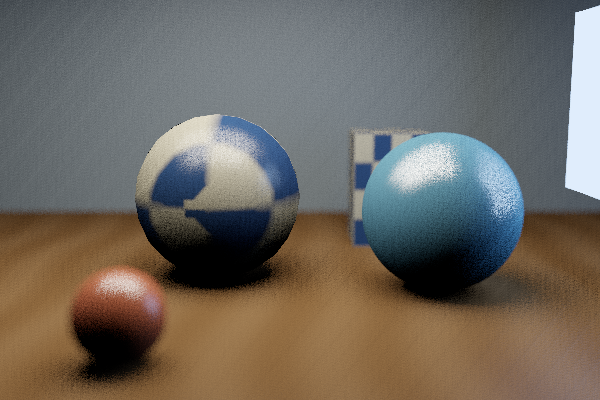
\includegraphics[width=0.8\textwidth]{DRT_simple.png}
    % Source: output/DRT_simple.png; 600x400, spp=32, aperture=0.18, focus=9.
    % Left checker sphere and background box are both OBJ meshes with UVs.
    \caption{DRT\_simple. The arrow points to the OBJ mesh (geodesic sphere) with smooth shading.}
    \label{fig:drt_simple}
\end{figure}
% 请自行补充：平滑着色与几何轮廓为何不同？

\subsection{Textures on Meshes}
\textbf{Design Decisions:} UV coordinates are interpolated using barycentric weights from the triangle intersection. The base color is computed as \( \text{DiffuseColor} \times \text{TextureAt}(\text{uv}) \).
\textbf{Example Render:}
In Figure \ref{fig:drt_simple}, the left OBJ mesh shows a blue/beige checkerboard texture.
% 请自行补充：为什么仅声明 texture 文件不够？

\subsection{Area Light Sources and Soft Shadows}
\textbf{Design Decisions:} I used PCG32 pseudo-random uniform sampling over the area light surface. The solid-angle PDF is \( r^2 / (\cos\theta_{\text{light}} \times A) \). The contribution per sample is \( f \times \cos\theta_{\text{surface}} \times L_e / \text{pdf} \times \text{beta} \), divided by the number of samples per light.
\textbf{Difficulties Encountered:} I initially mixed up the row/column coordinates of the rectangle emitter and forgot to transform the sampling normal to world space.
\textbf{Example Render:}
\begin{figure}[H]
    \centering
    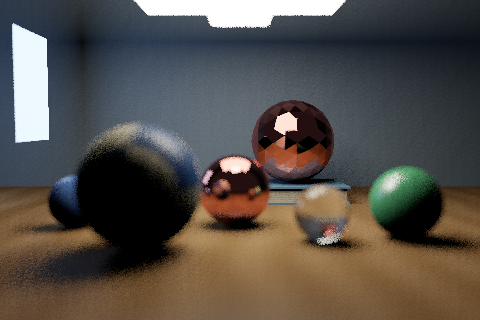
\includegraphics[width=0.8\textwidth]{DRT_creative.png}
    % Source: output/DRT_creative.png; 480x320, spp=24, aperture=0.18, focus=13.5.
    % TODO: add your real inspiration photograph and penumbra annotations.
    \caption{DRT\_creative. The arrow indicates the soft shadow (penumbra) cast by the green sphere.}
    \label{fig:drt_creative}
\end{figure}
% 请自行补充：部分光源可见如何产生半影？采样噪声和物理软阴影如何区分？

\subsection{Phong BRDF and Energy Conservation}
\textbf{Design Decisions:} The BRDF is \( k_d/\pi + k_s \frac{e+2}{2\pi} \max(0, \text{Reflect}(\mathbf{wi}, \mathbf{n}) \cdot \mathbf{wo})^e \), where \( k_s = \text{clamp}(\text{specular}, 0, 1) \) and \( k_d = \text{clamp}(\text{texturedDiffuse}, 0, 1) \times (1-k_s) \). The cosine term is multiplied in the integrator, not in the BRDF.
\textbf{Example Render:}
The glossy highlights on the balls in Figure \ref{fig:drt_creative} demonstrate the Phong BRDF.
% 请自行补充：lobe normalization 与总能量预算分别解决什么？

\subsection{Defocus Blur and Depth of Field}
\textbf{Design Decisions:} I implemented a thin-lens camera model. Lens sampling uses \( r = \text{lensRadius} \times \sqrt{u} \) and \( \theta = 2\pi v \). The focal point is \( \mathbf{p} + \mathbf{dir} \times t_f \), where \( t_f = \text{focusDistance} / (\mathbf{dir} \cdot \text{forward}) \).
\textbf{Difficulties Encountered:} I originally had each ray travel a fixed distance along its own direction, creating a spherical focal surface. I fixed this to intersect a flat focal plane.
\textbf{Example Render:}
In Figure \ref{fig:drt_simple} (aperture=0.18, focus=9.0), the foreground red ball and background box are blurred, while the mid-ground is sharp.
% 请自行补充：离焦与 sampling noise 的区别？A=0 时应怎样？

\subsection{Reinhard Tone Mapping}
% TODO: DRT_creative film max is 1.0; appearance alone does not prove no clipping.
\textbf{Design Decisions:} I used extended Reinhard tone mapping per RGB channel with white point \( W=8 \): \( c' = c \times (1 + c/W^2) / (1 + c) \). This is applied after averaging HDR samples and before sRGB encoding.
\textbf{Example Render:}
The white panels in Figure \ref{fig:drt_creative} are not blown out, demonstrating the tone mapping.
% 请自行补充：tone mapping 与 gamma/sRGB 有何不同？


\section{PBRT Scene Compatibility}
I support a subset of PBRT syntax including Film, Sampler, Integrator, LookAt, Camera, WorldBegin/End, Material, NamedMaterial, PPM imagemap Texture, point LightSource, diffuse AreaLightSource, sphere, inline trianglemesh, and basic transforms (Translate, Scale, Rotate).
\textbf{Error Handling:} The parser logs errors for missing textures or unknown shapes. Unsupported features (e.g., Includes, Object instances) are logged as warnings. A test fixture (\texttt{broken.pbrt}) confirms that the renderer handles errors gracefully without crashing.

\section{Profiling Results}
% 根据你的 txt 文件，这里只放 render time，并说明 parse/total timer 未完成
% TODO: final DRT measurements below were started concurrently; remeasure
% serially for a controlled baseline. The renderer itself is single-threaded.
The following table reports the render time for the four main scenes. Note that the parsing and total timers were not fully implemented at the time of this measurement, so only the render stage is reported. All timings are from a single-threaded run on an Apple M2 Pro.

\begin{table}[H]
    \centering
    \resizebox{\textwidth}{!}{%
    \begin{tabular}{lccccc}
        \toprule
        \textbf{Scene} & \textbf{Resolution} & \textbf{Samples/Pixel} & \textbf{Max Depth} & \textbf{Primitives} & \textbf{Render Time (s)} \\
        \midrule
        WSRT\_simple & 900x560 & 1 & 8 & 8 & 0.461692 \\
        WSRT\_creative & 960x600 & 1 & 12 & 47 & 3.801205 \\
        DRT\_simple & 600x400 & 32 & 4 & 336 & 66.585001 \\
        DRT\_creative & 480x320 & 24 & 4 & 682 & 82.613686 \\
        \bottomrule
    \end{tabular}
    }
    \caption{Render times for Module 1 scenes.}
    \label{tab:profiling}
\end{table}

\section{Conclusion}
In this module, I successfully implemented a Whitted-Style Ray Tracer and a Distributed Ray Tracer from scratch. The WSRT correctly handles specular reflection, refraction, Blinn-Phong shading, shadows, and textures. The DRT extends this with OBJ mesh loading, area light sampling for soft shadows, a Phong BRDF, depth of field, and Reinhard tone mapping.

The main difficulties were fixing the sign conventions for refraction and ensuring consistent \( t \) values after transformations. Future work will focus on adding a BVH acceleration structure (Module 3) to handle complex scenes more efficiently.

\end{document}
